% Options for packages loaded elsewhere
\PassOptionsToPackage{unicode}{hyperref}
\PassOptionsToPackage{hyphens}{url}
\documentclass[
  a4paper,
  twoside]{article}
\usepackage{xcolor}
\usepackage[margin=1.6in]{geometry}
\usepackage{amsmath,amssymb}
\setcounter{secnumdepth}{-\maxdimen} % remove section numbering
\usepackage{iftex}
\ifPDFTeX
  \usepackage[T1]{fontenc}
  \usepackage[utf8]{inputenc}
  \usepackage{textcomp} % provide euro and other symbols
\else % if luatex or xetex
  \usepackage{unicode-math} % this also loads fontspec
  \defaultfontfeatures{Scale=MatchLowercase}
  \defaultfontfeatures[\rmfamily]{Ligatures=TeX,Scale=1}
\fi
\usepackage{lmodern}
\ifPDFTeX\else
  % xetex/luatex font selection
\fi
% Use upquote if available, for straight quotes in verbatim environments
\IfFileExists{upquote.sty}{\usepackage{upquote}}{}
\IfFileExists{microtype.sty}{% use microtype if available
  \usepackage[]{microtype}
  \UseMicrotypeSet[protrusion]{basicmath} % disable protrusion for tt fonts
}{}
\usepackage{setspace}
\makeatletter
\@ifundefined{KOMAClassName}{% if non-KOMA class
  \IfFileExists{parskip.sty}{%
    \usepackage{parskip}
  }{% else
    \setlength{\parindent}{0pt}
    \setlength{\parskip}{6pt plus 2pt minus 1pt}}
}{% if KOMA class
  \KOMAoptions{parskip=half}}
\makeatother
\usepackage{color}
\usepackage{fancyvrb}
\newcommand{\VerbBar}{|}
\newcommand{\VERB}{\Verb[commandchars=\\\{\}]}
\DefineVerbatimEnvironment{Highlighting}{Verbatim}{commandchars=\\\{\}}
% Add ',fontsize=\small' for more characters per line
\usepackage{framed}
\definecolor{shadecolor}{RGB}{248,248,248}
\newenvironment{Shaded}{\begin{snugshade}}{\end{snugshade}}
\newcommand{\AlertTok}[1]{\textcolor[rgb]{0.94,0.16,0.16}{#1}}
\newcommand{\AnnotationTok}[1]{\textcolor[rgb]{0.56,0.35,0.01}{\textbf{\textit{#1}}}}
\newcommand{\AttributeTok}[1]{\textcolor[rgb]{0.13,0.29,0.53}{#1}}
\newcommand{\BaseNTok}[1]{\textcolor[rgb]{0.00,0.00,0.81}{#1}}
\newcommand{\BuiltInTok}[1]{#1}
\newcommand{\CharTok}[1]{\textcolor[rgb]{0.31,0.60,0.02}{#1}}
\newcommand{\CommentTok}[1]{\textcolor[rgb]{0.56,0.35,0.01}{\textit{#1}}}
\newcommand{\CommentVarTok}[1]{\textcolor[rgb]{0.56,0.35,0.01}{\textbf{\textit{#1}}}}
\newcommand{\ConstantTok}[1]{\textcolor[rgb]{0.56,0.35,0.01}{#1}}
\newcommand{\ControlFlowTok}[1]{\textcolor[rgb]{0.13,0.29,0.53}{\textbf{#1}}}
\newcommand{\DataTypeTok}[1]{\textcolor[rgb]{0.13,0.29,0.53}{#1}}
\newcommand{\DecValTok}[1]{\textcolor[rgb]{0.00,0.00,0.81}{#1}}
\newcommand{\DocumentationTok}[1]{\textcolor[rgb]{0.56,0.35,0.01}{\textbf{\textit{#1}}}}
\newcommand{\ErrorTok}[1]{\textcolor[rgb]{0.64,0.00,0.00}{\textbf{#1}}}
\newcommand{\ExtensionTok}[1]{#1}
\newcommand{\FloatTok}[1]{\textcolor[rgb]{0.00,0.00,0.81}{#1}}
\newcommand{\FunctionTok}[1]{\textcolor[rgb]{0.13,0.29,0.53}{\textbf{#1}}}
\newcommand{\ImportTok}[1]{#1}
\newcommand{\InformationTok}[1]{\textcolor[rgb]{0.56,0.35,0.01}{\textbf{\textit{#1}}}}
\newcommand{\KeywordTok}[1]{\textcolor[rgb]{0.13,0.29,0.53}{\textbf{#1}}}
\newcommand{\NormalTok}[1]{#1}
\newcommand{\OperatorTok}[1]{\textcolor[rgb]{0.81,0.36,0.00}{\textbf{#1}}}
\newcommand{\OtherTok}[1]{\textcolor[rgb]{0.56,0.35,0.01}{#1}}
\newcommand{\PreprocessorTok}[1]{\textcolor[rgb]{0.56,0.35,0.01}{\textit{#1}}}
\newcommand{\RegionMarkerTok}[1]{#1}
\newcommand{\SpecialCharTok}[1]{\textcolor[rgb]{0.81,0.36,0.00}{\textbf{#1}}}
\newcommand{\SpecialStringTok}[1]{\textcolor[rgb]{0.31,0.60,0.02}{#1}}
\newcommand{\StringTok}[1]{\textcolor[rgb]{0.31,0.60,0.02}{#1}}
\newcommand{\VariableTok}[1]{\textcolor[rgb]{0.00,0.00,0.00}{#1}}
\newcommand{\VerbatimStringTok}[1]{\textcolor[rgb]{0.31,0.60,0.02}{#1}}
\newcommand{\WarningTok}[1]{\textcolor[rgb]{0.56,0.35,0.01}{\textbf{\textit{#1}}}}
\usepackage{longtable,booktabs,array}
\usepackage{calc} % for calculating minipage widths
% Correct order of tables after \paragraph or \subparagraph
\usepackage{etoolbox}
\makeatletter
\patchcmd\longtable{\par}{\if@noskipsec\mbox{}\fi\par}{}{}
\makeatother
% Allow footnotes in longtable head/foot
\IfFileExists{footnotehyper.sty}{\usepackage{footnotehyper}}{\usepackage{footnote}}
\makesavenoteenv{longtable}
\usepackage{graphicx}
\makeatletter
\newsavebox\pandoc@box
\newcommand*\pandocbounded[1]{% scales image to fit in text height/width
  \sbox\pandoc@box{#1}%
  \Gscale@div\@tempa{\textheight}{\dimexpr\ht\pandoc@box+\dp\pandoc@box\relax}%
  \Gscale@div\@tempb{\linewidth}{\wd\pandoc@box}%
  \ifdim\@tempb\p@<\@tempa\p@\let\@tempa\@tempb\fi% select the smaller of both
  \ifdim\@tempa\p@<\p@\scalebox{\@tempa}{\usebox\pandoc@box}%
  \else\usebox{\pandoc@box}%
  \fi%
}
% Set default figure placement to htbp
\def\fps@figure{htbp}
\makeatother
\ifLuaTeX
  \usepackage{luacolor}
  \usepackage[soul]{lua-ul}
\else
  \usepackage{soul}
\fi
% definitions for citeproc citations
\NewDocumentCommand\citeproctext{}{}
\NewDocumentCommand\citeproc{mm}{%
  \begingroup\def\citeproctext{#2}\cite{#1}\endgroup}
\makeatletter
 % allow citations to break across lines
 \let\@cite@ofmt\@firstofone
 % avoid brackets around text for \cite:
 \def\@biblabel#1{}
 \def\@cite#1#2{{#1\if@tempswa , #2\fi}}
\makeatother
\newlength{\cslhangindent}
\setlength{\cslhangindent}{1.5em}
\newlength{\csllabelwidth}
\setlength{\csllabelwidth}{3em}
\newenvironment{CSLReferences}[2] % #1 hanging-indent, #2 entry-spacing
 {\begin{list}{}{%
  \setlength{\itemindent}{0pt}
  \setlength{\leftmargin}{0pt}
  \setlength{\parsep}{0pt}
  % turn on hanging indent if param 1 is 1
  \ifodd #1
   \setlength{\leftmargin}{\cslhangindent}
   \setlength{\itemindent}{-1\cslhangindent}
  \fi
  % set entry spacing
  \setlength{\itemsep}{#2\baselineskip}}}
 {\end{list}}
\usepackage{calc}
\newcommand{\CSLBlock}[1]{\hfill\break\parbox[t]{\linewidth}{\strut\ignorespaces#1\strut}}
\newcommand{\CSLLeftMargin}[1]{\parbox[t]{\csllabelwidth}{\strut#1\strut}}
\newcommand{\CSLRightInline}[1]{\parbox[t]{\linewidth - \csllabelwidth}{\strut#1\strut}}
\newcommand{\CSLIndent}[1]{\hspace{\cslhangindent}#1}
\setlength{\emergencystretch}{3em} % prevent overfull lines
\providecommand{\tightlist}{%
  \setlength{\itemsep}{0pt}\setlength{\parskip}{0pt}}
% chrisdoc fonts not found
% This is where the typesetting magic happens
% Please don't judge my latex - I'm an R person not a latex person
% I took a problem solving approach (ok i want to do this, next I want to do this)
% So it might not necessarily be the most coherent code
% and its cobbled together from a variety of places (mostly stack overflow)
% plus some help from AI

% Font settings

\usepackage{fontspec}
\defaultfontfeatures{Ligatures=TeX,Scale=MatchLowercase}

\setmainfont{SourceSerif4-Regular.ttf}[
  Path=\chrisdocfontpath,
  BoldFont=SourceSerif4-Bold.ttf,
  ItalicFont=SourceSerif4-Italic.ttf,
  BoldItalicFont=SourceSerif4-BoldItalic.ttf
]

\setsansfont{SourceSans3-Regular.ttf}[
  Path=\chrisdocfontpath,
  BoldFont=SourceSans3-Bold.ttf,
  ItalicFont=SourceSans3-Italic.ttf,
  BoldItalicFont=SourceSans3-BoldItalic.ttf,
  SemiboldFont=SourceSans3-Semibold.ttf,
  SemiboldItalicFont=SourceSans3-SemiboldItalic.ttf
]

% Stuff for typewrite fonts
\defaultfontfeatures{Scale=MatchLowercase}
\defaultfontfeatures[\rmfamily]{Ligatures=TeX}
\defaultfontfeatures[\sffamily]{Ligatures=TeX}

\setmonofont{SourceCodePro-Regular.ttf}[
  Path=\chrisdocfontpath,
  BoldFont=SourceCodePro-Bold.ttf,
  ItalicFont=SourceCodePro-Italic.ttf,
  RawFeature={-liga,-clig,-calt}
]

\usepackage{unicode-math}
\setmathfont{STIXTwoMath-Regular.ttf}[
Path=\chrisdocfontpath
]



% Font size + line spacing
\fontsize{12pt}{15.6pt}\selectfont

% Icons for cover page
\usepackage{fontawesome5}

% Footnote indentings
\usepackage[hang]{footmisc}      % already have this
\setlength{\footnotemargin}{.5em} % your preferred indent

% Tighter footnote vertical spacing
\setlength{\footnotesep}{0.5\baselineskip} % default ~0.6

% Reduce paragraph skip within a footnote
\setlength{\skip\footins}{6pt plus 2pt minus 1pt} % space above footnotes
\renewcommand{\footnotelayout}{\setlength{\parskip}{0pt}}

% Extra stuff for annoying cover page footnotes
\usepackage{etoolbox}
\makeatletter
\let\fm@makefntext\@makefntext
\patchcmd\maketitle{\if@twocolumn}{\let\@makefntext\fm@makefntext\if@twocolumn}{}{\fail}
\makeatother

% List spacing
\usepackage{enumitem}
\setlist{topsep = 0pt, itemsep = 0pt}

% Make all tabular environments use sans font by default

\AtBeginEnvironment{tabular}{\sffamily}
\AtBeginEnvironment{longtable}{\sffamily}
\AtBeginEnvironment{threeparttable}{\sffamily}
\AtBeginEnvironment{tabu}{\sffamily}
\AtBeginEnvironment{longtabu}{\sffamily}

\usepackage{siunitx}

% Make number columns follow the surrounding font and styles
\sisetup{
  detect-mode = true,
  detect-family = true,
  detect-weight = true,
  detect-shape = true
}

% Title stuff
\makeatletter

% Title fonts
\newfontfamily\TitleSans{SourceSans3-Semibold.ttf}[
  Path = \chrisdocfontpath,
  ItalicFont = SourceSans3-SemiboldItalic.ttf
]
\newfontfamily\SubtitleFont{SourceSans3-Regular.ttf}[
  Path = \chrisdocfontpath,
  BoldFont = SourceSans3-Bold.ttf,
  ItalicFont = SourceSans3-Italic.ttf,
  BoldItalicFont = SourceSans3-BoldItalic.ttf,
  LetterSpace = 1.5
]

% Title block spacing
\patchcmd{\@maketitle}{\begin{center}}{\begin{center}\vspace*{10em}}{}{}


% Title and subtitle formatting
\patchcmd{\@maketitle}{\@title}{{\TitleSans\fontsize{24}{6}\selectfont \@title}}{}{}

\providecommand{\subtitle}[1]{%
  \apptocmd{\@title}{%
    \par\vspace{0.15em}%
    {\SubtitleFont\LARGE #1}%
    \par\vspace{0.35em}%
  }{}{}%
}

\makeatother

% Abstract formatting

\makeatletter
\renewenvironment{abstract}{%
  \par\vspace{0.25\baselineskip}%
  \begingroup\setlength{\parindent}{0pt}\noindent\ignorespaces
}{%
  \par\endgroup\vspace{0.5\baselineskip}%
  \thispagestyle{cover}%
  \clearpage
  \pagenumbering{arabic}\setcounter{page}{1}%
}
\makeatother


% Title page note formatting
\makeatletter

% Take out date from title block
\patchcmd{\@maketitle}{\@date}{}{}{}

% Default if no TitlePageNote
\@ifundefined{TitlePageNote}{\newcommand{\TitlePageNote}{}}{}%

% Add extra notes after the author notes
\providecommand{\markerlessthanks}[1]{%
  \protected@xdef\@thanks{\@thanks\protect\footnotetext[0]{#1}}%
}

\patchcmd{\@maketitle}{\@author}{%
  \@author

  % TitlePageNote
  \ifx\TitlePageNote\@empty\else
    \markerlessthanks{\vspace*{-0.5\baselineskip}}
    \markerlessthanks{\TitlePageNote}%
  \fi
  % Version
  \ifx\@date\@empty\else
    \markerlessthanks{\vspace*{-0.5\baselineskip}}
    \markerlessthanks{\textbf{This version:} \@date}%
  \fi
}{}{}

\makeatother


% Cover status header stuff
\usepackage{xcolor}
\usepackage{fancyhdr}

\providecommand{\coverstatus}{}

\fancypagestyle{cover}{%
  \fancyhf{}%
  \renewcommand{\headrulewidth}{0pt}%
  \setlength{\headheight}{14pt}% ensure room for the header
  \lhead{%
    {\sffamily\scshape\color{black!60}\fontsize{11}{12}\selectfont \coverstatus}%
  }%
}


\makeatletter
\pretocmd{\@maketitle}{\thispagestyle{cover}}{}{}
\makeatother


% Section header formatting
\usepackage{titlesec}

% Fonts
\titleformat{\section}
  {\sffamily\bfseries\Large}
  {\thesection}{0.75em}{}

\titleformat{\subsection}
  {\sffamily\bfseries\large}
  {\thesubsection}{0.6em}{}

\titleformat{\subsubsection}
 {\sffamily\fontseries{sb}\selectfont\normalsize}
 {\thesubsubsection}{0.5em}{}

% Spacing: left, before, after
\titlespacing*{\section}{0pt}{.8\baselineskip plus .2\baselineskip minus .2\baselineskip}{.2\baselineskip}
\titlespacing*{\subsection}{0pt}{0.4\baselineskip plus .1\baselineskip minus .1\baselineskip}{.1\baselineskip}
\titlespacing*{\subsubsection}{0pt}{0.2\baselineskip plus .05\baselineskip minus .05\baselineskip}{0\baselineskip}


% Captions
\usepackage{caption}
\usepackage{subcaption}

% Define a semibold font for caption labels
\DeclareCaptionFont{sb}{\fontseries{sb}\selectfont}

% Global caption style
\captionsetup{
  font       = {sf,small},
  labelfont  = {sf,sb},
  format     = plain,
  singlelinecheck = true, % controls short captions being centred
  labelsep   = colon,  % alternatives: period | space | endash | quad | newline
}

% Caption position
\captionsetup[table]{position=above}
\captionsetup[figure]{position=below}

% Subfigures formatted the same
\captionsetup[sub]{font={sf,small}, labelfont={sf,sb}, labelsep=colon}

% Stuff for appendix titling
\makeatletter

\newcommand{\MainTitle}{}

\AtBeginDocument{%
  \begingroup
  \long\def\extractfirst#1\par#2\END{\gdef\MainTitle{#1}}%
  \expandafter\extractfirst\@title\par\END
  \endgroup
}
\makeatother


% Fancy pagecount
\usepackage{lastpage}

\makeatletter
\AtBeginDocument{%
  \renewcommand{\headrulewidth}{0pt}%
  \renewcommand{\footrulewidth}{0pt}%

  % Main text: fancy or normal page number
  \fancypagestyle{fancy-main}{%
    \fancyhf{}%
    \ifdefined\usefancypagecount
      \fancyfoot[C]{Page \thepage\ of \pagerefLastMain}%
    \else
      \fancyfoot[C]{\thepage}%
    \fi
  }%

  % Appendix: fancy or normal page number
  \fancypagestyle{fancy-apdx}{%
    \fancyhf{}%
    \ifdefined\usefancypagecount
      \fancyfoot[C]{Appendix page \thepage\ of \pageref{LastPageAppendix}}%
    \else
      \fancyfoot[C]{\thepage}%
    \fi
  }%

  \pagestyle{fancy-main}%
}

% Capture appendix position and do page numbering things
\pretocmd{\appendix}{%
  \label{LastPageMain}
  \clearpage

  \setcounter{page}{1}%
  \ifdefined\usefancypagecount
    \renewcommand{\thepage}{\arabic{page}}%
    \providecommand{\theHpage}{}%
    \renewcommand{\theHpage}{app.\arabic{page}}%
  \else
    \renewcommand{\thepage}{A\arabic{page}}%
    \providecommand{\theHpage}{}%
    \renewcommand{\theHpage}{A\arabic{page}}%
  \fi

  \pagestyle{fancy-apdx}%
}{}{}

% Define last page depending on whether there's an appendix
\usepackage{lastpage}

\makeatletter
\newcommand*\pagerefLastMain{%
  \ifcsname r@LastPageMain\endcsname
    \pageref{LastPageMain}%
  \else
    \pageref{LastPage}%
  \fi}
\makeatother


% Headers - fill them in from the yaml
\providecommand{\MainHeaderOdd}{}
\providecommand{\MainHeaderEven}{}
\providecommand{\ApdxHeaderOdd}{}
\providecommand{\ApdxHeaderEven}{}

% If you want a headrule, change this in header-includes:
\providecommand{\SetHeadruleWidth}{0pt}

\makeatletter
\AtBeginDocument{%
  \renewcommand{\headrulewidth}{\SetHeadruleWidth}%
  \renewcommand{\footrulewidth}{0pt}%

% Header fonts
\fancypagestyle{fancy-main}{%
  \fancyhf{}%
  \fancyhead[CO]{\sffamily\scshape\color{black!60}\fontsize{11}{12}\selectfont \MainHeaderOdd}%
  \fancyhead[CE]{\sffamily\scshape\color{black!60}\fontsize{11}{12}\selectfont \MainHeaderEven}%
  % Clear the other header positions
  \fancyhead[LO,LE,RE,RO]{}%

  % Page formatting
  \ifdefined\usefancypagecount
    \fancyfoot[C]{\sffamily\scshape\color{black!60}\fontsize{11}{12}\selectfont{Page \thepage\ of \pagerefLastMain}}%
  \else
    \fancyfoot[C]{\thepage}%
  \fi
}%

% Appendix headers and page nubmers
\fancypagestyle{fancy-apdx}{%
  \fancyhf{}%

  \fancyhead[CO]{\sffamily\scshape\color{black!60}\fontsize{11}{12}\selectfont \ApdxHeaderOdd}%
  \fancyhead[CE]{\sffamily\scshape\color{black!60}\fontsize{11}{12}\selectfont \ApdxHeaderEven}%
  \fancyhead[LO,LE,RO,RE]{}%

  \ifdefined\usefancypagecount
    \fancyfoot[C]{\sffamily\scshape\color{black!60}\fontsize{11}{12}\selectfont {Appendix page \thepage\ of \pageref{LastPageAppendix}}}%
  \else
    \fancyfoot[C]{\thepage}%
  \fi
}%
  \pagestyle{fancy-main}%
}
\makeatother


% For demonstrating the header font
\newcommand{\headerdemo}[1]{{\sffamily\scshape\color{black!60}\fontsize{11}{12}\selectfont #1}}


% Label the final appendix page for page numbering
\AtEndDocument{\label{LastPageAppendix}}
\makeatother

% Custom code chunk colours
% Normal, 12 colours from https://tsitsul.in/blog/coloropt/
\definecolor{yellow}{rgb}{0.92,0.67,0.14}   % #ebac23
\definecolor{lipstick}{rgb}{0.72,0.00,0.35} % #b80058
\definecolor{azure}{rgb}{0.00,0.55,0.98}    % #008cf9
\definecolor{green}{rgb}{0.00,0.43,0.00}    % #006e00
\definecolor{caribbean}{rgb}{0.00,0.73,0.68}% #00bbad
\definecolor{lavender}{rgb}{0.82,0.39,0.90} % #d163e6
\definecolor{brown}{rgb}{0.70,0.27,0.01}    % #b24502
\definecolor{coral}{rgb}{1.00,0.57,0.53}    % #ff9287
\definecolor{indigo}{rgb}{0.35,0.33,0.84}   % #5954d6
\definecolor{turquoise}{rgb}{0.00,0.78,0.97}% #00c6f8
\definecolor{olive}{rgb}{0.53,0.52,0.00}    % #878500
\definecolor{jade}{rgb}{0.00,0.65,0.42}     % #00a76c
\definecolor{gray}{rgb}{0.74,0.74,0.74}     % #bdbdbd
\definecolor{black}{rgb}{0.00,0.00,0.00}   % #000000


% Background

\definecolor{shadecolor}{RGB}{248, 250, 252}

% Colour mapping
% Safe remaps for Pandoc highlighting macros — only redefine if they exist
\makeatletter
\@ifundefined{AlertTok}{}{\renewcommand{\AlertTok}[1]{\textcolor{lipstick}{\textbf{#1}}}}
\@ifundefined{AnnotationTok}{}{\renewcommand{\AnnotationTok}[1]{\textcolor{lipstick}{\textbf{\textit{#1}}}}}
\@ifundefined{AttributeTok}{}{\renewcommand{\AttributeTok}[1]{\textcolor{black}{#1}}}
\@ifundefined{BaseNTok}{}{\renewcommand{\BaseNTok}[1]{\textcolor{black}{#1}}}
\@ifundefined{BuiltInTok}{}{\renewcommand{\BuiltInTok}[1]{#1}}
\@ifundefined{CharTok}{}{\renewcommand{\CharTok}[1]{\textcolor{green}{#1}}}
\@ifundefined{CommentTok}{}{\renewcommand{\CommentTok}[1]{\textcolor{lipstick}{\textit{#1}}}}
\@ifundefined{CommentVarTok}{}{\renewcommand{\CommentVarTok}[1]{\textcolor{lipstick}{\textbf{\textit{#1}}}}}
\@ifundefined{ConstantTok}{}{\renewcommand{\ConstantTok}[1]{\textcolor{lipstick}{#1}}}
\@ifundefined{ControlFlowTok}{}{\renewcommand{\ControlFlowTok}[1]{\textcolor{azure}{\textbf{#1}}}}
\@ifundefined{DataTypeTok}{}{\renewcommand{\DataTypeTok}[1]{\textcolor{azure}{#1}}}
\@ifundefined{DecValTok}{}{\renewcommand{\DecValTok}[1]{\textcolor{black}{#1}}}
\@ifundefined{DocumentationTok}{}{\renewcommand{\DocumentationTok}[1]{\textcolor{lipstick}{\textbf{\textit{#1}}}}}
\@ifundefined{ErrorTok}{}{\renewcommand{\ErrorTok}[1]{\textcolor{yellow}{\textbf{#1}}}}
\@ifundefined{ExtensionTok}{}{\renewcommand{\ExtensionTok}[1]{#1}}
\@ifundefined{FloatTok}{}{\renewcommand{\FloatTok}[1]{\textcolor{black}{#1}}}
\@ifundefined{FunctionTok}{}{\renewcommand{\FunctionTok}[1]{\textcolor{azure}{#1}}}
\@ifundefined{ImportTok}{}{\renewcommand{\ImportTok}[1]{#1}}
\@ifundefined{InformationTok}{}{\renewcommand{\InformationTok}[1]{\textcolor{lipstick}{\textbf{\textit{#1}}}}}
\@ifundefined{KeywordTok}{}{\renewcommand{\KeywordTok}[1]{\textcolor{azure}{\textbf{#1}}}}
\@ifundefined{NormalTok}{}{\renewcommand{\NormalTok}[1]{#1}}
\@ifundefined{OperatorTok}{}{\renewcommand{\OperatorTok}[1]{\textcolor{black}{\textbf{#1}}}}
\@ifundefined{OtherTok}{}{\renewcommand{\OtherTok}[1]{\textcolor{lipstick}{#1}}}
\@ifundefined{PreprocessorTok}{}{\renewcommand{\PreprocessorTok}[1]{\textcolor{lipstick}{\textit{#1}}}}
\@ifundefined{RegionMarkerTok}{}{\renewcommand{\RegionMarkerTok}[1]{#1}}
\@ifundefined{SpecialCharTok}{}{\renewcommand{\SpecialCharTok}[1]{\textcolor{black}{\textbf{#1}}}}
\@ifundefined{SpecialStringTok}{}{\renewcommand{\SpecialStringTok}[1]{\textcolor{green}{#1}}}
\@ifundefined{StringTok}{}{\renewcommand{\StringTok}[1]{\textcolor{green}{#1}}}
\@ifundefined{VariableTok}{}{\renewcommand{\VariableTok}[1]{\textcolor{black}{#1}}}
\@ifundefined{VerbatimStringTok}{}{\renewcommand{\VerbatimStringTok}[1]{\textcolor{green}{#1}}}
\@ifundefined{WarningTok}{}{\renewcommand{\WarningTok}[1]{\textcolor{lipstick}{\textbf{\textit{#1}}}}}
\makeatother


% For landscape pages
\usepackage{pdflscape}
\newcommand{\blandscape}{\begin{landscape}}
\newcommand{\elandscape}{\end{landscape}}

% For the appendix table of contents
\usepackage{titletoc}

% If \MainTitle isn't already defined
\providecommand{\MainTitle}{\thetitle}

% Appendix title page malarky
\newcommand{\AppendixAutoSetup}{%
  \newpage
  \thispagestyle{empty}%
  % numbering depth for sections/ToC in appendix
  \setcounter{secnumdepth}{3}%
  \setcounter{tocdepth}{3}%
  % Appendix labels A1, A2, ... for sections, figures, tables, equations
  \renewcommand{\thesection}{A\arabic{section}}%
  \renewcommand{\thefigure}{A\arabic{figure}}%
  \setcounter{figure}{0}%
  \renewcommand{\thetable}{A\arabic{table}}%
  \setcounter{table}{0}%
  \renewcommand{\theequation}{A\arabic{equation}}%
  \setcounter{equation}{0}%
  % Title block
  \begin{center}
    {\sffamily\Large Appendix to\par}
    \vspace{0.4em}
    {\sffamily\bfseries\LARGE \MainTitle\par}
  \end{center}
  % Appendix TOC
  \startcontents[appendixtoc]%
  \begingroup
    \renewcommand{\contentsname}{\vspace{-2em}}%
    \titlecontents{section}[0em]
      {\addvspace{1em}}
      {\makebox[1em][l]{\thecontentslabel}\hspace{1em}}
      {}
      {\titlerule*[0.5pc]{.}\contentspage}
    \titlecontents{subsection}[2em]
      {\addvspace{0.5em}}
      {\makebox[2em][l]{\thecontentslabel}\hspace{1em}}
      {}
      {\titlerule*[0.5pc]{.}\contentspage}
    \titlecontents{subsubsection}[5em]
      {\addvspace{0.5em}}
      {\makebox[3em][l]{\thecontentslabel}\hspace{1em}}
      {}
      {\titlerule*[0.5pc]{.}\contentspage}
    \printcontents[appendixtoc]{1}{1}{\subsection*{\contentsname}}%
  \endgroup
  \newpage
  \setcounter{page}{1}%
}

% Apply to \appendix switch
\apptocmd{\appendix}{\AppendixAutoSetup}{}{\fail}

\renewcommand{\coverstatus}{Template example}
\renewcommand{\TitlePageNote}{The cover page has space for three types of footnotes (1) author information, (2) acknowledgements etc (this bit of text), and (3) version date. The icons come from \texttt{fontawesome5}, which includes thousands of icons, including useful ones such as ORCID \faOrcid\ and GitHub \faGithub, and more frivolous ones you could use to indicate the paper was written on a beach \faUmbrellaBeach.}
\def\usefancypagecount{}
\renewcommand{\MainHeaderOdd}{The chrisdoc R Markdown template}
\renewcommand{\MainHeaderEven}{Template example}
\renewcommand{\ApdxHeaderOdd}{Appendix to the chrisdoc R Markdown template}
\renewcommand{\ApdxHeaderEven}{Template example appendix}
\renewcommand{\SetHeadruleWidth}{0pt}
\usepackage{float}
\floatplacement{table}{H}
\usepackage{tikz, tikz-cd}\usetikzlibrary{arrows.meta}\newcommand{\longdashleftrightarrow}[1][1.75em]{\mathrel{\tikz[baseline]{\draw[dash pattern=on 0.25em off 0.1 em,<->](0,.58ex)--(#1,.58ex)}}}
\usepackage{booktabs}
\usepackage{longtable}
\usepackage{array}
\usepackage{multirow}
\usepackage{wrapfig}
\usepackage{float}
\usepackage{colortbl}
\usepackage{pdflscape}
\usepackage{tabu}
\usepackage{threeparttable}
\usepackage{threeparttablex}
\usepackage[normalem]{ulem}
\usepackage{makecell}
\usepackage{xcolor}
\usepackage{siunitx}

    \newcolumntype{d}{S[
      table-align-text-before=false,
      table-align-text-after=false,
      input-symbols={-,\*+()}
    ]}
  
\usepackage{bookmark}
\IfFileExists{xurl.sty}{\usepackage{xurl}}{} % add URL line breaks if available
\urlstyle{same}
\hypersetup{
  pdftitle={The Chrisdoc R Markdown Template},
  pdfauthor={Christopher Prosser},
  hidelinks,
  pdfcreator={LaTeX via pandoc}}

\title{The Chrisdoc R Markdown Template}
\usepackage{etoolbox}
\makeatletter
\providecommand{\subtitle}[1]{% add subtitle to \maketitle
  \apptocmd{\@title}{\par {\large #1 \par}}{}{}
}
\makeatother
\subtitle{Custom typsetting, plus handy bits of code}
\author{Christopher Prosser\footnote{\faUniversity~Royal Holloway, University of London\newline
  \faGlobe~\href{https://caprosser.com/}{caprosser.com}\newline
  \faEnvelope~\href{mailto:chris.prosser@rhul.ac.uk}{chris.prosser@rhul.ac.uk}}}
\date{30 October 2025}

\begin{document}
\maketitle
\begin{abstract}
This is an R Markdown template for writing academic papers. This document explains the template and demonstrates its typography. This bit of the paper is what the abstract looks like. \newline \newline \textbf{Keywords:} R Markdown; Typography; Template
\end{abstract}

\setstretch{1}
This is a \texttt{R\ Markdown} template for writing academic papers and turning them into pdfs. It aims to produces elegantly and professionally typeset documents with minimal fuss at the writing stage. This document serves both as a explanation and example of the template design. The typesetting happens by adding a \LaTeX~preamble to \texttt{bookdown::pdf\_document2} and settings in the \texttt{yaml}. The \texttt{Rmd} part of the template also contains code for things such plots, tables, and Ti\emph{k}Z diagrams that are not necessary for typesetting but (a) show what different things look like using the template, and (b) I use all the time, so it is useful for me to put them all in one place.

\section{Why bother making and using a template?}\label{why-bother-making-and-using-a-template}

This is a question I asked myself many times when this ended up taking much longer than I thought it would.\footnote{Thanks \LaTeX \ldots

  Since this is the first footnote, it seems the appropriate place to note that footnotes are indented to the right of their footnote marker (and not the default hanging indent approach).}

The short answer is I like things that look nice; I think this looks nice. There are plenty of existing templates out there, many of them look good, none of them look quite how I wanted.

The more intellectual answer is that as much as we might wish that our readers would judge our work on the basis of its content, aesthetics matter. Nice typography can put people in a better mood (Larson et al. 2007). Perceptual fluency influences judgments about truth (Reber and Schwarz 1999). Good design can influence assessments of scholarly interest and scientific rigour (Cheng et al. 2022). You might as well put your best foot forward.

Mostly though, I just like things to look nice.

\section{Installation and use}\label{installation-and-use}

I made this template for my own use, but if you also write things in \texttt{R\ Markdown}, feel free to use it too. If you do use the template, please let me know---that would make my day. If you don't like it, don't tell me---make your own.

You can find the template on \texttt{GitHub} here: \href{https://github.com/drcaprosser/chrisdoc}{github.com/drcaprosser/chrisdoc}. In \texttt{R} you can install the template like so:

\begin{quote}
\texttt{remotes::install\_github("drcaprosser/chrisdoc")}
\end{quote}

There are two versions of the template in the package, a `max' version, which has all the typesetting plus bits of example code, and a `min' version, which is just a blank document with the typesetting elements.

Since I made this for my own use, the author field is pre-populated with my information. If you end up using it on a regular basis you might want to fork the \texttt{GitHub} repository and edit the \texttt{.Rmd} files to put your own information in.

Also since I made this for my own use, a disclaimer: please consider the template to be in perpetual beta---I might change my mind on things such as fonts in the future, and will implement those changes if I feel like it. I'll try not to make any breaking changes---I don't want to break my own old projects---but no guarantees.

At some point I'll probably port this over to \texttt{Quarto} but because of a combination of path dependency (\texttt{R\ Markdown} does what I want it to, and I have used it for years) and some equivalent functions being missing in \texttt{R\ Studio} (specifically, the inability to load a template via File \rightarrow~New File \rightarrow~Quarto Document), I'm sticking with \texttt{R\ Markdown} for now.

\section{The template design}\label{the-template-design}

Typesetting is driven by my own aesthetic preferences, strongly influenced by \emph{Butterick's Practical Typography}.\footnote{\url{https://practicaltypography.com/}} One obvious feature of the template is the relatively wide margins. There are good reasons for this. As Butterick puts it:

\begin{quote}
Shorter lines are more comfortable to read than longer lines. As line length increases, your eye has to travel farther from the end of one line to the beginning of the next, making it harder to track your progress vertically. Aim for an average line length of 45--90 characters, including spaces.
\end{quote}

Using the default (1.6 inch) margins, a block of \emph{Lorem ipsum} boilerplate has a mean line length of 89.25 characters. I originally made the margins even wider, but it squished the plots too much. Large margins also leave plenty of rooms for scribbling notes.

Font choice and line spacing are based on recommendations from Butterick. The main font is Source Serif 4. Headings and captions use \textsf{Source Sans~3}. Code chunks and the like use \texttt{Source\ Code\ Pro}. Butterick doesn't have any recommendations for maths fonts, but \(STIX \ Two \ Math\) looks nice to me, so I've used that. The main font is 12pt, and default line spacing is 130\% of that.

The text is fully justified, and uses hyphenation for long words that run across line breaks. It also uses hanging punctuation (i.e.~punctuation that occurs at the end of a line is set slightly outside the margin to create a clean edge). These are all inherited from \texttt{bookdown::pdf\_document2}, but I would have set them this way manually if they were not.

Section and subsection headers are unnumbered by default (though that is easy to change in the \texttt{yaml}), appear in bold, with extra space around them to denote a break in text (with decreasing font size and space as you move down the header hierarchy).

\section{Headers}\label{headers}

The template includes the option to have different headers on odd and even pages. These are set via some short code in \texttt{header-includes} bit of the \texttt{yaml}. If you don't want headers, you can leave them blank. Headers are typeset in \headerdemo{grey small-caps Source Sans~3}. By default there is no headrule, but if you want one you can edit the \texttt{SetHeadruleWidth} bit of code in the \texttt{header-includes} bit of the \texttt{yaml}.

\section{Page numbers}\label{page-numbers}

There are two options for page numbering:

\begin{enumerate}
\def\labelenumi{\arabic{enumi}.}
\item
  `Fancy' \headerdemo{Page x of y} style numbers, typeset the same way as the headers.
\item
  Ordinary numerals (1, 2, 3 etc).\footnote{Since this is a list, this seems like a good place to note that the template uses slightly more compact list spacing than the defaults.}
\end{enumerate}

To turn off fancy page numbers, just get rid of the \texttt{usefancypagecount} line from the \texttt{header-includes} bit of the \texttt{yaml}.

\section{Figures}\label{figures}

By default, \texttt{ggplot2} figures are drawn using \texttt{theme\_academic} from my \texttt{chrisplot} package, which follows similar \st{stylistic prejudices} aesthetic principles as this template, and also uses \textsf{Source Sans~3}, so hopefully they look nice together.\footnote{See: \href{https://github.com/drcaprosser/chrisplot}{github.com/drcaprosser/chrisplot}.

  To install: \texttt{remotes::install\_github("drcaprosser/chrisplot")}.}

The setup chunk contains a bunch of functions and chunk options that control figures size based on page size/margins and the golden ratio. The purpose of this code is to align figures nicely with the text and make the fonts the same size as the text. \texttt{chrisplot} uses very narrow plot margins, so plots should take up nearly all of the space between the page margins. I wanted to make the plot margins zero, so it took up all of the space, but the lower right x-axis label tended to get clipped off. I might figure out a solution to this at some point.

Potentially my most controversial choice regarding figures is that they do not float. I understand the arguments for floating from a typographical perspective---it minimises unnecessary white space, which looks ugly. But as a \emph{reader} I have always found floated figures and tables irritating---coming across a floated figure before it is mentioned in the text breaks the flow of reading, as does searching high and low for a table that has been floated beyond the horizon. Floating also devalues the role of figures and tables in academic writing---they are not mere decoration but key to scientific reporting. You wouldn't float the paragraphs setting out your theory; don't float your figures.\footnote{This doesn't mean I think you should ignore whitespace problems---you should try to avoid them as much as possible. But such problems are better solved by a bit of thought about where a figure should appear, rather than relying on an algorithm.}

Figure captions use \textsf{Source Sans~3}, with the caption type and number bolded and followed by a colon. Captions are justified differently depending on the length of the caption. Figure \ref{fig:aplot} shows a plot with a long caption, and figure \ref{fig:anotherplot} shows a plot with a short caption. Figure \ref{fig:fullpageplot} show a full portrait page plot while figure \ref{fig:alandplot} shows a full landscape page plot. Full page plots need manually set chunk \texttt{fig.asp} options to look nice. The template R Markdown has further comments about the aspect ratios that fit the default margins.

\begin{figure}[H]

{\centering 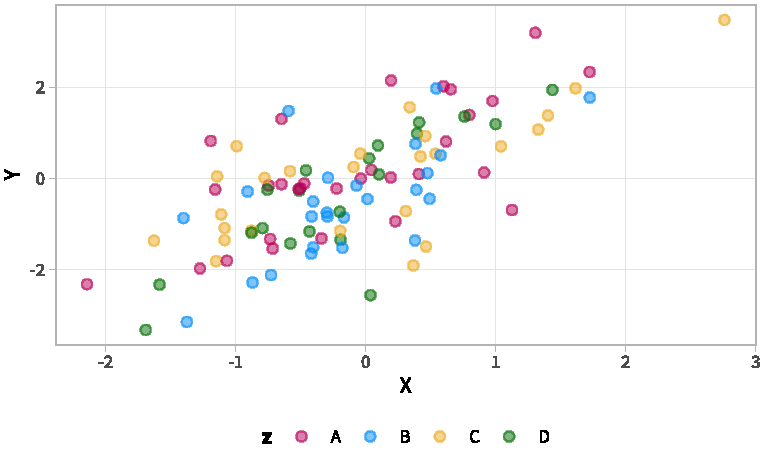
\includegraphics[width=\linewidth,]{chrisdoc_example_files/figure-latex/aplot-1} 

}

\caption{This is a plot with a long caption. Sometimes captions need to have lots of information in them. Mostly that is because plots need proper explanation, particularly because people often skip to them first rather than waiting till they get to the relevant part of the paper. Othertimes you need a long captions because a style guide has dictated you need to re-explain your legend in text form. When captions run longer than one line, as this one does, captions are fully justified.}\label{fig:aplot}
\end{figure}

\begin{figure}[H]

{\centering 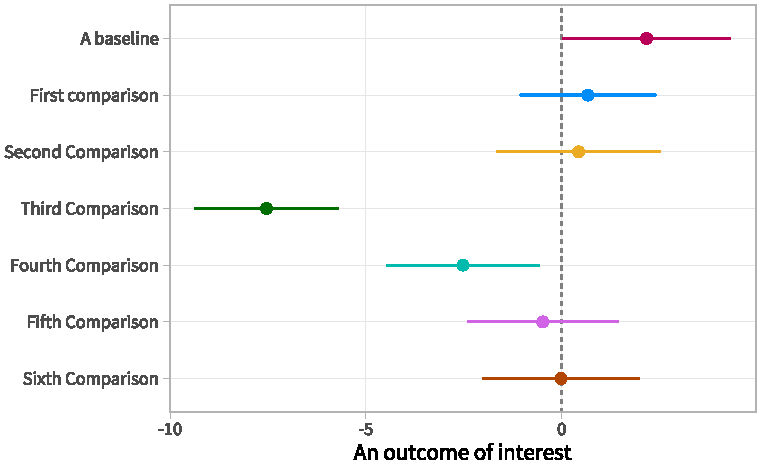
\includegraphics[width=\linewidth,]{chrisdoc_example_files/figure-latex/anotherplot-1} 

}

\caption{Short captions are centered.}\label{fig:anotherplot}
\end{figure}

\begin{figure}[H]

{\centering 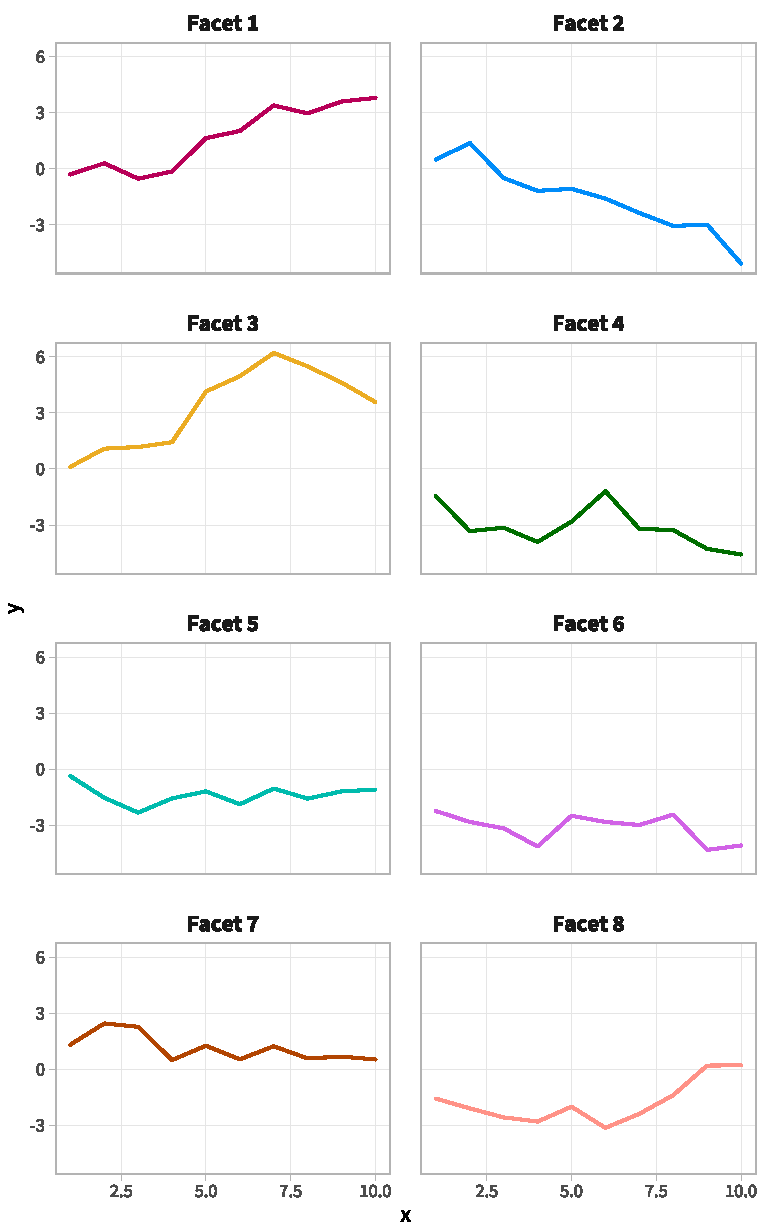
\includegraphics[width=\linewidth,]{chrisdoc_example_files/figure-latex/fullpageplot-1} 

}

\caption{A plot that takes up a full page.}\label{fig:fullpageplot}
\end{figure}

\blandscape

\begin{figure}[H]

{\centering 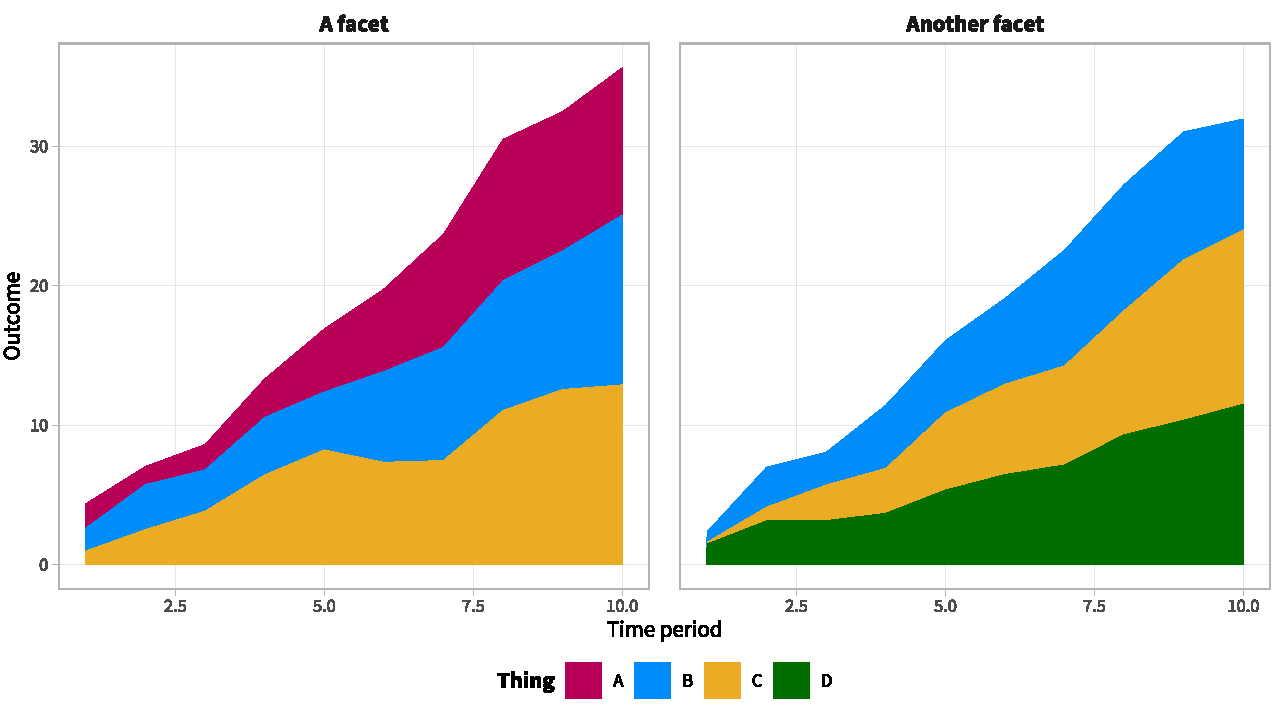
\includegraphics[width=\linewidth,]{chrisdoc_example_files/figure-latex/alandplot-1} 

}

\caption{This is a plot on a landscape page. }\label{fig:alandplot}
\end{figure}

\elandscape

\section{Tables}\label{tables}

I generally use \texttt{kable} and \texttt{kableExtra} to make tables. The \texttt{kable} and \texttt{kableExtra} packages use the unmaintained and apparently broken \texttt{tabu} \LaTeX~package, so at some point I'll start using something else. The most likely candidate is \texttt{tinytable}, because Vincent Arel-Bundock's other packages (\texttt{modelsummary} and \texttt{marginaleffects}) are amazing and I use them all the time, but I'll have to figure out how to do the things I already know how to do with \texttt{kable}, so for now I'm staying put\ldots

Tables are typeset in \textsf{Source Sans~3}, as shown in table \ref{tab:atable}.

Like figures, tables do not float. Table captions have the same style as figure captions.

\begin{table}

\caption{\label{tab:atable}This is a table.}
\centering
\begin{tabular}[t]{lrrrr}
\toprule
\multicolumn{1}{c}{ } & \multicolumn{2}{c}{Numbers} & \multicolumn{2}{c}{Decimals} \\
\cmidrule(l{3pt}r{3pt}){2-3} \cmidrule(l{3pt}r{3pt}){4-5}
Letters & Some numbers & More numbers & Some decimals & More decimals\\
\midrule
A & 1 & 8 & 1.00 & 0.12\\
B & 2 & 9 & 0.50 & 0.11\\
C & 3 & 10 & 0.33 & 0.10\\
D & 4 & 11 & 0.25 & 0.09\\
E & 5 & 12 & 0.20 & 0.08\\
F & 6 & 13 & 0.17 & 0.08\\
G & 7 & 14 & 0.14 & 0.07\\
\bottomrule
\end{tabular}
\end{table}

I use \texttt{modelsummary} to make regression tables, using the \texttt{kableExtra} backend, which produces output like that shown in table \ref{tab:regtable}.

\begin{table}
\centering
\caption{\label{tab:regtable}This is a regression table with a long caption to demonstrate the text justification behaviour of captions. The models show a classic observational research pattern.}
\centering
\begin{tabular}[t]{lddd}
\toprule
\multicolumn{1}{c}{ } & \multicolumn{2}{c}{Bivariate} & \multicolumn{1}{c}{Multivariate} \\
\cmidrule(l{3pt}r{3pt}){2-3} \cmidrule(l{3pt}r{3pt}){4-4}
  & {(1)} & {(2)} & {(3)}\\
\midrule
Key variable for your theory & 0.51*** & {} & -0.02\\
 & (0.03) & {} & (0.03)\\
Some annoying confound & {} & 1.03*** & 1.05***\\
 & {} & (0.03) & (0.05)\\
Intercept & -0.02 & -0.03 & -0.03\\
 & (0.04) & (0.03) & (0.03)\\
\midrule
N & \multicolumn{1}{c}{1000} & \multicolumn{1}{c}{1000} & \multicolumn{1}{c}{1000}\\
$R^2$ & \multicolumn{1}{c}{0.26} & \multicolumn{1}{c}{0.52} & \multicolumn{1}{c}{0.52}\\
\bottomrule
\multicolumn{4}{l}{\rule{0pt}{1em}+ p $<$ 0.1, * p $<$ 0.05, ** p $<$ 0.01, *** p $<$ 0.001}\\
\end{tabular}
\end{table}

\section{Maths}\label{maths}

Equation \eqref{eq:egeq} shows some maths. This is a changepoint model that comes from a paper I co-authored about class voting in Britain from 1885--2024 that is currently under review, I put it here so you can see what the font looks like.

\begin{equation}
\label{eq:egeq}
y_t = \alpha + \beta_0 t + \sum_{j=1}^{n} \beta_j (t - \text{cp}_j) \cdot \mathbb{I}(t > \text{cp}_j) + \epsilon_t
\end{equation}

\section{\texorpdfstring{Ti\emph{k}Z}{TikZ}}\label{tikz}

Occasionally, I use Ti\emph{k}Z to draw diagrams, mostly Directed Acyclic Graphs (DAGs), like figure \ref{fig:urdag}, which shows a DAG illustrating the problem with making causal claims about just about everything. To draw DAGs I use \href{https://q.uiver.app/}{\emph{q.uiver.app}} and then drop the Ti\emph{k}Z code into the document.

\begin{figure}[H]
\centering
\begin{tikzcd}
    && U \\
    \\
    x &&&& y
    \arrow[dashed, from=1-3, to=3-1]
    \arrow[dashed, from=1-3, to=3-5]
    \arrow[from=3-1, to=3-5]
\end{tikzcd}
\caption{The Ur-DAG}
\label{fig:urdag}
\end{figure}

\section{Appendices}\label{appendices}

The template includes code to create an appendix section at the end of the document, which inserts a cover page, pipes in the title of the paper from the \texttt{yaml} and adds a table of contents. The appendix uses separate section, figure, table and page numbering to the main document. Having an appendix in the same document makes cross referencing easy. See for example, figure \ref{fig:appendixplot} in appendix \ref{appendixOne}.

To start the appendix, just put

\begin{quote}
\texttt{\textbackslash{}appendix}
\end{quote}

in the body of the Rmd after the reference section.

The appendix has the option for different headers on odd and even pages that are separate to the main text. It also uses slightly different page numbering styles. With fancy page numbering you get \begingroup \sffamily\scshape\color{black!60}\fontsize{11}{12}\selectfont
Appendix page x of y%
\endgroup\ and with ordinary page numbering you get numerals prefixed with an 'A' (A1, A2, A3 etc). 

When you submit something to a journal you generally have to submit the appendix as a separate file, but it is easy to split a pdf file up. There is some code in appendix \ref{appendixPDFsplit} to help you do that, which also shows the template's custom code highlighting theme, which uses the same colour palette as the default \texttt{chrisplot} palette.

\newpage

Here is a page of boilerplate text so you can see the different levels of section and subsection headings.

\section{A section}\label{a-section}

Lorem ipsum dolor sit amet, consectetur adipiscing elit, sed do eiusmod tempor incididunt ut labore et dolore magna aliqua. Ut enim ad minim veniam, quis nostrud exercitation ullamco laboris nisi ut aliquip ex ea commodo consequat. Duis aute irure dolor in reprehenderit in voluptate velit esse cillum dolore eu fugiat nulla pariatur. Excepteur sint occaecat cupidatat non proident, sunt in culpa qui officia deserunt mollit anim id est laborum.

Lorem ipsum dolor sit amet, consectetur adipiscing elit, sed do eiusmod tempor incididunt ut labore et dolore magna aliqua. Ut enim ad minim veniam, quis nostrud exercitation ullamco laboris nisi ut aliquip ex ea commodo consequat. Duis aute irure dolor in reprehenderit in voluptate velit esse cillum dolore eu fugiat nulla pariatur. Excepteur sint occaecat cupidatat non proident, sunt in culpa qui officia deserunt mollit anim id est laborum.

\subsection{A subsection}\label{a-subsection}

Lorem ipsum dolor sit amet, consectetur adipiscing elit, sed do eiusmod tempor incididunt ut labore et dolore magna aliqua. Ut enim ad minim veniam, quis nostrud exercitation ullamco laboris nisi ut aliquip ex ea commodo consequat. Duis aute irure dolor in reprehenderit in voluptate velit esse cillum dolore eu fugiat nulla pariatur. Excepteur sint occaecat cupidatat non proident, sunt in culpa qui officia deserunt mollit anim id est laborum.

Lorem ipsum dolor sit amet, consectetur adipiscing elit, sed do eiusmod tempor incididunt ut labore et dolore magna aliqua. Ut enim ad minim veniam, quis nostrud exercitation ullamco laboris nisi ut aliquip ex ea commodo consequat. Duis aute irure dolor in reprehenderit in voluptate velit esse cillum dolore eu fugiat nulla pariatur. Excepteur sint occaecat cupidatat non proident, sunt in culpa qui officia deserunt mollit anim id est laborum.

\subsubsection{A subsubsection}\label{a-subsubsection}

Lorem ipsum dolor sit amet, consectetur adipiscing elit, sed do eiusmod tempor incididunt ut labore et dolore magna aliqua. Ut enim ad minim veniam, quis nostrud exercitation ullamco laboris nisi ut aliquip ex ea commodo consequat. Duis aute irure dolor in reprehenderit in voluptate velit esse cillum dolore eu fugiat nulla pariatur. Excepteur sint occaecat cupidatat non proident, sunt in culpa qui officia deserunt mollit anim id est laborum.

Lorem ipsum dolor sit amet, consectetur adipiscing elit, sed do eiusmod tempor incididunt ut labore et dolore magna aliqua. Ut enim ad minim veniam, quis nostrud exercitation ullamco laboris nisi ut aliquip ex ea commodo consequat. Duis aute irure dolor in reprehenderit in voluptate velit esse cillum dolore eu fugiat nulla pariatur. Excepteur sint occaecat cupidatat non proident, sunt in culpa qui officia deserunt mollit anim id est laborum.

\newpage

\section*{References}\label{references}
\addcontentsline{toc}{section}{References}

\phantomsection\label{refs}
\begin{CSLReferences}{1}{0}
\bibitem[\citeproctext]{ref-cheng2022}
Cheng, Karen, Yeechi Chen, Kevin Larson, and Marco Rolandi. 2022. {``Proving the Value of Visual Design in Scientific Communication.''} \emph{Information Design Journal}, July, 80--95. \url{https://doi.org/10.1075/idj.23.1.09che}.

\bibitem[\citeproctext]{ref-larson}
Larson, Kevin, Richard L. Hazlett, Barbara S. Chaparro, and Rosalind W. Picard. 2007. {``Measuring the Aesthetics of Reading.''} In, 41--56. Springer London. \url{https://doi.org/10.1007/978-1-84628-664-3_4}.

\bibitem[\citeproctext]{ref-reber1999}
Reber, Rolf, and Norbert Schwarz. 1999. {``Effects of Perceptual Fluency on Judgments of Truth.''} \emph{Consciousness and Cognition} 8 (3): 338--42. \url{https://doi.org/10.1006/ccog.1999.0386}.

\end{CSLReferences}

\appendix

\section{Example appendix}\label{appendixOne}

Here's an appendix with an extra plot in it.

\begin{figure}[H]

{\centering 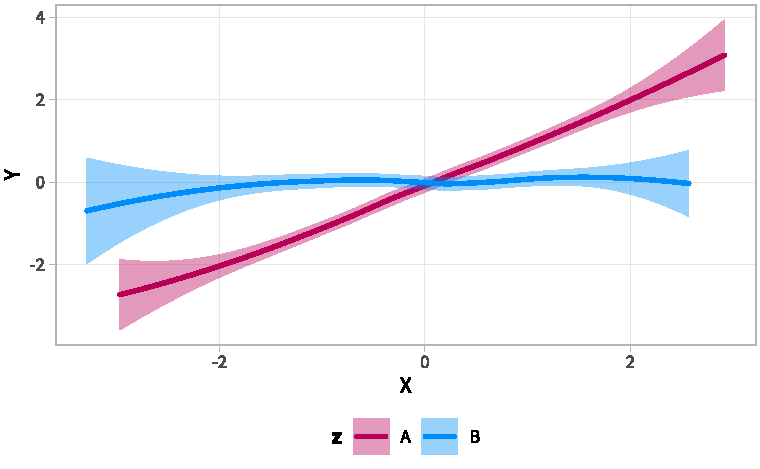
\includegraphics[width=\linewidth,]{chrisdoc_example_files/figure-latex/appendixplot-1} 

}

\caption{This is a plot in the appendix.}\label{fig:appendixplot}
\end{figure}

\newpage

\section{PDF splitting code}\label{appendixPDFsplit}

Here's some code to split a pdf into different parts. Copy this into an \texttt{R} script and edit the file paths and names to match your documents.

\begin{Shaded}
\begin{Highlighting}[]
\CommentTok{\# Split pdfs into main text and appendices}

\FunctionTok{library}\NormalTok{(pdftools)}

\NormalTok{pdf\_file }\OtherTok{\textless{}{-}} \StringTok{"file\_path\_to\_your\_document\_here.pdf"}
\NormalTok{pdf\_text }\OtherTok{\textless{}{-}} \FunctionTok{pdf\_text}\NormalTok{(pdf\_file)}

\CommentTok{\# Find first page of appendix}

\NormalTok{target\_page }\OtherTok{\textless{}{-}} \FunctionTok{grep}\NormalTok{(}\StringTok{"Appendix to"}\NormalTok{, pdf\_text)[}\DecValTok{1}\NormalTok{]}

\CommentTok{\# Split document into title page, main document, and appendix}

\CommentTok{\# Standalone title page}

\FunctionTok{pdf\_subset}\NormalTok{(pdf\_file,}
           \AttributeTok{pages =} \DecValTok{1}\SpecialCharTok{:}\DecValTok{1}\NormalTok{, }
           \AttributeTok{output =} \StringTok{"title\_page.pdf"}\NormalTok{)}

\CommentTok{\# Main document}
\CommentTok{\# If you need it without the title page}
\CommentTok{\# Set \textasciigrave{}pages = 2:(target\_page{-}1)\textasciigrave{}}

\FunctionTok{pdf\_subset}\NormalTok{(pdf\_file,}
           \AttributeTok{pages =} \DecValTok{1}\SpecialCharTok{:}\NormalTok{(target\_page}\DecValTok{{-}1}\NormalTok{), }
           \AttributeTok{output =} \StringTok{"main\_document.pdf"}\NormalTok{)}

\CommentTok{\# Appendix}

\FunctionTok{pdf\_subset}\NormalTok{(pdf\_file,}
           \AttributeTok{pages =}\NormalTok{ target\_page}\SpecialCharTok{:}\FunctionTok{length}\NormalTok{(pdf\_text), }
           \AttributeTok{output =} \StringTok{"appendix.pdf"}\NormalTok{)}
\end{Highlighting}
\end{Shaded}


\end{document}
